\documentclass[12pt]{article}
\addtolength{\oddsidemargin}{-2cm}
\addtolength{\evensidemargin}{-2cm}
\addtolength{\textwidth}{4cm}

\addtolength{\topmargin}{-2cm}
\addtolength{\textheight}{3cm}

\usepackage[usenames, dvipsnames]{color}
\usepackage{amsmath}
\usepackage{amssymb}
\usepackage{enumitem}
\usepackage{float}
\usepackage{enumitem}

\usepackage{graphicx}
\usepackage[utf8]{inputenc}
\usepackage{hyperref}
\hypersetup{
	colorlinks=true,
	linkcolor=blue,
	filecolor=magenta,      
	urlcolor=cyan,
}

\usepackage{listings}
\usepackage{xcolor}
\lstset{
	frame=tb, % draw a frame at the top and bottom of the code block
	tabsize=4, % tab space width
	showstringspaces=false, % don't mark spaces in strings
	numbers=left, % display line numbers on the left
	commentstyle=\color{green}, % comment color
	keywordstyle=\color{blue}, % keyword color
	stringstyle=\color{red} % string color
}

\begin{document}

\thispagestyle{empty}
\begin{titlepage}
	\null\vfill
	
	\begin{center}
		
		{\Huge Cammott-Boids Project Report}
		\vskip 2cm
		
		{\large CPSC 565 University of Calgary}
	\end{center}
	
	\vfill
	\vfill
	
	\begin{tabular}{r}
		Camilo Talero\ \\
		Scott Saunders\    
	\end{tabular}
	\hfill
\end{titlepage}

	
\newpage
\clearpage
\setcounter{page}{1}

\section*{Abstract}

\indent We implemented an interactive C++ program that displays multiple flocks of simple agents (called Boids in honour of the original paper by Craig Reynolds). The program uses user-editable text files to create different groups of Boids with different behaviours, and spawns obstacles, represented as spheres, that the Boids must avoid. Boids can also be controlled by the user by point and clicking.
\\ \\
Boids are governed by the 3 rules originally described by Reynolds (cohesion, separation and alignment). Cohesion is the desire of each Boid to go to the average position of its neighbours; separation is the desire of the agents to prevent collisions by moving away from neighbours; alignment is the desire to match the general heading of their neighbours. Some modifications were also added, such as the addition of a field of view. Each rule is independent and each can be configured via the text file.
\\ \\
Boids are a good example of emergent systems, since each agent is very simplistic in nature, yet complex behaviours can be achieved through modifications of a small set of parameters. They are the basis for many swarm simulations, such as the bats in the BAFTA nominated film Batman Begins, which, along other things, was nominated for its special effects.

\section{Overview}
\subsection{Basic Rules}
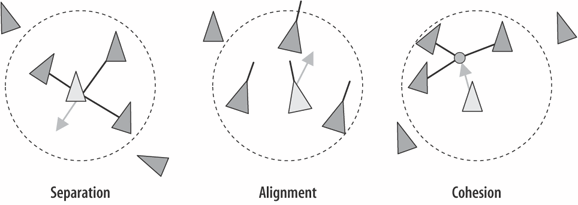
\includegraphics[width=\textwidth,height=\textheight,keepaspectratio]{rules.png}
\subsubsection{Separation}
The separation rule governs the desire to avoid collisions of the Boids. There are 2 parameters that directly affect this rule.
\\ \\
The \textbf{sepRadius} parameter governs the radius of a sphere placed around the center of mass of the Boid that is used to determine which Boids affect the current Boid. The \textbf{sepCoeff} parameter governs the strength with which Boids repel each other. All Boids outside of this sphere will be ignored. The current Boid will calculate the average position of all Boids inside of its separation sphere of radius, \textbf{sepRadius}, and will attempt to move away from this position with an acceleration magnitude of \textbf{sepCoeff}.

\subsubsection{Alignment}
The alignment rule governs the desire of a Boid to match the general heading of its neighbours. There are 2 parameters that directly influence this rule.
\\ \\
The \textbf{alignmentRadius} parameter determines the radius of a sphere around the center of mass of the Boid that is used to determine which Boids affect the current Boid. The \textbf{alignmentCoeff} determines the strength of the force with which Boids accelerate to match the general heading of its neighbours. The current Boid will ignore all Boids outside of this sphere, it will then calculate the average heading of all Boids that are inside of its alignment sphere but outside of its separation sphere (which forces the alignment sphere to always be bigger than the separation sphere if this rule is to be applied) and then it will accelerate so that its heading matches that of its neighbours with a magnitude of \textbf{alignmentCoff}.

\subsubsection{Cohesion}
The cohesion rule governs the desire of a Boid to head towards the general position of its neighbours. There are 2 parameters that directly influence this rule.
\\ \\
The \textbf{cohesionRadius} determines the radius of the sphere around the center of mass of the Boid that is used to determine which Boids affect the current Boid. The \textbf{cohesionCoeff} parameter determines the magnitude of the force with which the current Boid  accelerates towards the average position of its neighbours inside of the cohesion sphere. All Boids outside the cohesion sphere as well as those inside the alignment or separation spheres will be ignored (forcing the radius of this sphere to be larger than that of the previous to for this rule to take effect).

\subsubsection{Field of view}
There is an additional rule that determines whether a Boid can see another Boid or not. If the current Boid cannot see a Boid, even if this Boid is inside any of the rule spheres (cohesion, alignment and separation) it will be ignored. There is only one parameter affecting this rule.
\\ \\
\textbf{FOV} determines the field of view of all Boids in a flock. The simplest way to abstract this rule is to imagine that inside each of the rule spheres described above, there is a conic hole of angle $(360 - \textbf{FOV})$, any Boid that lies inside of this conic section will be ignored by the current Boid regardless of its position.

\subsection{Additional rules}
\subsubsection{Herding (attractive and repelling)}
This is an additional rule that allows the user to herd a flock towards/away to/from a point through the use of the mouse. There are no user configurable parameters associated with this rule.
\\ \\
If the user presses the left mouse button, the average position of the flock is approximated by sampling 20 Boids from the current flock. The current position of the mouse is then projected onto the 3D world with the same depth as this approximated position. All Boids in the current flock then accelerate towards this projected point, until the user let's go of the button.
\\ \\
If the user presses the right mouse button, similar calculations are performed, except the Boid gets repelled from the projected point.
\subsubsection{Keep Territory}
This rule creates a territory for the flocks (same for all flocks, but could be implemented so that it is flock specific in the future). This creates a desire for all flocks to avoid going too far away from the starting position. There is 1 parameter associated with this rule.
\\ \\
\textbf{radius} determines the radius of a territory sphere centres at the origin $O=(0,0,0)$. If a Boid wanders outside this territory (i.e the length of its position radius exceeds radius), It will ignore all other rules and will accelerate towards the origin. This essentially ensures that neither Boids nor flocks stray into infinity.

\subsubsection{Collision Avoidance}
This rule ensures Boids won't collide with the spherical obstacles added to the world. There are no user-editable parameters associated with this  rule.
\\ \\
If a Boid passes a threshold distance (not user configurable) it will get repelled away from the center of the collision sphere with a magnitude of $k\cdot \frac{1}{distance^2}$ for a constant, implementation specific $k$, where distance refers to the distance form the Boid to the surface of the collision sphere. This ensures that the closer the Boid is to a collision sphere, the stronger it will be repelled away from it, and as such this force eventually overcomes the forces of any other rule if the Boid gets too close to the sphere.

\subsection{Additional parameters}
\begin{itemize}
	\item \textbf{BoidNum}: the number of Boids of the flock.
	\item \textbf{color}: the color of the Boids in the flock (purely for aesthetic purposes).
	\item \textbf{center}: not fully implemented, no behaviour. Once implemented, determines the center of the territory of the flock.
	\item \textbf{maxAcceleration}: this parameter prevents the Boids from changing their velocity too fast. The current magnitude of the acceleration experienced by a Boid may never exceed \textbf{maxAcceleration}. If it does the net acceleration's magnitude gets changed accordingly so that it becomes \textbf{maxAcceleration}.
	\item \textbf{maxVelocity}: this parameter prevents the Boids from reaching velocities that are too fast. Same as with acceleration, if the velocity vector's magnitude of a Boid would exceed this value, it gets changed accordingly so as to not exceed it. 
\end{itemize}

\section{Implementation}
The entire project was coded using C++. The libraries OpenGL, GLM, and GLEW are also used, both for rendering and simulation purposes. There will be no discussion about the implementation of the basic rules described on the Overview, as this has been widely discussed in other places. For an example of a possible pseudo-code of each rule please refer to: \url{http://www.kfish.org/Boids/pseudocode.html}.
\\ \\
We profited from the multi-paradigmatic nature of C++ and used both its procedural programming and object orientation aspects to structure the simulation. In particular, the simulation itself runs as a procedural program, and there is no object orientation neither on the main cpp file nor on the main loop of the program. However Flocks, Boids, and collision objects were all represented as cpp objects with their respective header files. And all behaviour of their behaviour was encoded as member functions of their class representations (e.g the behaviour rules are functions inside the Boid class). 

\subsection{Optimization Techniques}
The most important optimization technique implemented was a technique to sub divide the space using a hash table. A cube of side length \textbf{radius} (a cube capable of containing the territory sphere) is created. This space is then sub-divided and all Boids are mapped to the sub-volume they lie on. Each sub-volume is then hashed using the the $i,j,k$ values of its front, lower, left corner.
\\ \\
\noindent The following code snippets show the functions directly involved with the space hashing. The hash table is represented as a vector of vectors of Boid pointers, since each bucket in the hash table must contain all Boids inside the voxel mapped to that position on the hash table. Each flock has its own hash table, included in its class definition.

\begin{minipage}[t]{\textwidth}
\begin{lstlisting}[language=C++]
//hashFunction
void Flock::hash(Boid* b)
{
	if(hashTable.size() == 0)
		hashTable.resize(Boids.size()*2);
	
	uint hashIndex = b->x*LP1+ b->y*LP2 + b->z*LP3;
	hashIndex = hashIndex%hashTable.size();
	uint originalHI = hashIndex;
	
	while(hashTable[hashIndex].size()>0 &&
	(hashTable[hashIndex][0]->x!=b->x ||
	hashTable[hashIndex][0]->y!=b->y ||
	hashTable[hashIndex][0]->z!=b->z))
	{
		hashIndex = (hashIndex+1)%(hashTable.size());
		if(hashIndex == originalHI)
			return;
	}

	hashTable[hashIndex].push_back(b);
}
\end{lstlisting}
\end{minipage}

\begin{minipage}[t]{\textwidth}
\begin{lstlisting}[language=C++]
//voxelize the space and the Boids
void Flock::allocate()
{
	for(Boid *b: Boids)
	{
		int x = (b->position.x+radius)/cohesionRadius;
		int y = (b->position.y+radius)/cohesionRadius;
		int z = (b->position.z+radius)/cohesionRadius;
		
		b->x=x;
		b->y=y;
		b->z=z;
		
		hash(b);
	}
}
\end{lstlisting}
\end{minipage}

Although the worst case running time of the previous algorithm is $O(n^2)$, the same running time as no optimization. The use of the hash table makes it so that, as long as the Boids are not too close to each other, the amortized running time is $O(n)$ (where n is the number of Boids).
\\ \\

Two further optimization techniques were implemented. 
\\ \\
The first, was to parallelize the simulation via pthreads when updating the Boids. The number of concurrent threads is guaranteed to be the maximum number of concurrent threads that can run simultaneously on the current CPU (machine independent). Instead of updating each Boid on one thread, the Boids get separated into \textit{number of concurrent threads} equal sized partitions and each thread updates only those Boids associated to it. So all threads may read the information of any Boid, but can only write to those Boids associated to it, thus ensuring consistency.
\\ \\
The second was to increment CPU time by requesting a higher priority to the operating system. If the program is run with administration privileges (e,g run with the use of sudo in Ubuntu) it will request the operating system to give it the maximum priority (-20). However, depending on the CPU load this may have little to no impact on the simulation. The priority with which the program is running is displayed on the console at the beginning of the execution.
\\ \\
These optimization techniques allowed us to have up to 10 000 Boids in 1 flock, with acceptable lag. It is however recommended to keep the number of Boids at around 5000 to prevent unexpected lag when a large number of Boids clusters together.

\subsection{Mathematical Model}
\subsubsection{Physics and Numerical Integration}
In order to have a smooth and realistic looking simulation, our approach to simulate each Boid is based on physics. The abstraction is to consider each Boid as a particle that can be affected by certain physical forces. We assumed all Boids had the same mass thus we simplified Newton's second law of motion, $F=ma$, to simply $F=a$ or in other words, Boids accelerate based exclusively on the forces being applied to them. Each of the rules discussed in the overview section generates a vector, representing a force that is to be applied to the current Boid. 
\\ \\
At a given time $t$ this yields $a_t = \sum a_r$ where $a_t$ is the acceleration at time $t$ and $\{a_r\}$ is the set of all accelerations calculated by the behaviour rules. 
\\ \\
This approach has the advantage that any arbitrary amount of rules can be added in a very simple manner. However it may be necessary to increase \textbf{maxAcceleration} and \textbf{maxVelocity} when doing so.
\\ \\
Finally, we update all parameters defined in the Boid class, following the Verlet integration approach. In other words we follow the formula:
$$X_{t+\Delta t} = X_t + (X_t-X_{t_{past}})\cdot(\frac{\Delta t}{\Delta t_{past}}) + a_t\cdot(\frac{\Delta t + \Delta t_{past}}{2})\cdot\Delta t$$
Where the \textit{past} subscript denotes the value of that variable on the previous time step\\
$t_{past}=t-\Delta t$, and $X_t$ denotes the position of the Boid at time $t$.
\\ \\
Similarly, we update the velocity of the Boid to be: 
$$v_{t+\Delta t} = \frac{X_{t+\Delta t} - X_{t_{past}}}{2\Delta t}$$

The choice of this specific numerical integration approach was not arbitrary. This Verlet integration approach does not require a constant time step, making it very suitable for real-time simulations, since, ideally, if the CPU lags, the simulation does not lag along with it, but rather it gets updated based on the real time value of $t$, calculated since the beginning of the execution of the program. The downside is that, due to the nature of numerical integration, a significant lag in the computer may lead to big errors in calculations.

\subsubsection{Asynchronous Error Elimination}
The reader may have noted that updating each Boid one after the other creates an error in the simulation, that propagates and becomes larger which each new updated void. Simply, if on a given time step $t$ a Boid's position is changed, then all Boids that depended on this Boid are affected as well (e.g imagine a Boid moves away form the visual range of one of its neighbours before they neighbour is updated, then the neighbour will not behave appropriately based on the state of the world on the current time step). To avoid this the above calculations are performed for each Boid and the results are stored.  Each Boid is then updated after all calculations are performed. This prevents the error propagation described above.

\subsubsection{Boid Orientation}
Since this simulation focuses on visual aspects, it is important that the Boids behave in a seemingly natural way. To ensure that each Boid faces in the direction of its velocity, the approach is quite simple. We take the current heading of the Boid and its current velocity and normalize both. Then we cross product the 2 to obtain the normal to the plain containing the 2 vectors, and we finally rotate the geometry of the Boid, around this normal by the angle in between the 2 vectors. More formally:

$$\hat{n}=\vec{d}\times \vec{v}$$
$$\theta = acos(\vec{d}\cdot\vec{v})$$

Once the above values are obtained we construct the corresponding rotation matrix and rotate each point in the Boid geometry by it.

\section{Results}
The purpose of this simulation was to create flocks of simple agents that behaved in ways that look realistic and interesting. It is not a scientific simulation of real animals, as such, the success of the project is relative to the apparent complexity of the flocks, rather than to any numerical value, statistical data or real life comparison with real animals. 
\\ \\
Based on the above, the final result consists of a group of flocks, each composed of 1000 Boids with the default parameters and a set of collision spheres spread around randomly in the world.
Each Boid has a color in order to identify which flock it belongs to, so as to make it easier to observe any emergence in the simulation. This allows us to see the first result of the project. 
\\ \\
At the beginning of the simulation, all Boids are evenly distributed across the space. There are no clusters nor groups of Boids on the very first moments of the simulation. However, we can see that, as time progresses, Boids of matching color (i.e Boids belonging to the same flock) Have a tendency of grouping together, and we can easily see clear, distinct Boid congregations appear over time. 
\\ \\
Moreover, it is evident to the viewer, that, given the parameters provided with the original simulation (the original text files of the simulation before any modification by the user) Each color of Boid (each flock) has its own unique behaviour, even if some are similar. On this set of parameters (available on a GitHub repository of the project, provided at the end of this document) we can describe the following behaviours per color. \\
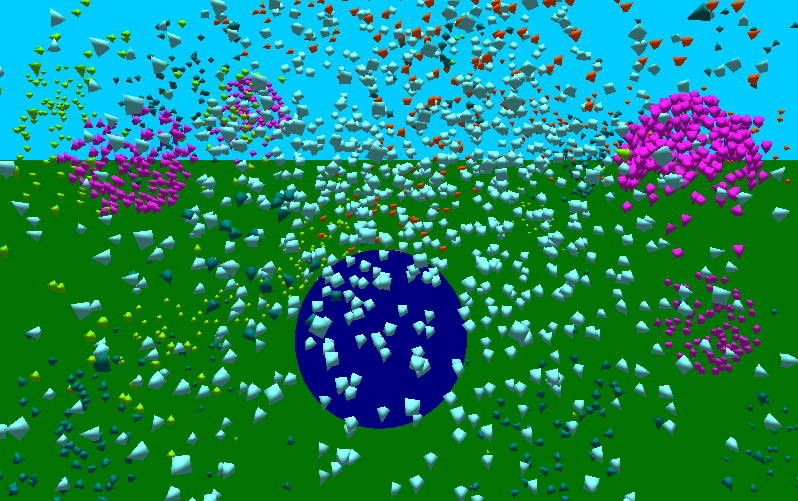
\includegraphics[width=\textwidth,height=\textheight,keepaspectratio]{small.png}
\\
\begin{itemize}
	\item Orange: creates groups of Boids that move together as a whole, but each Boid still moves about.
	
	\item Green: Creates groups, possibly dense, mostly out of alignment, and will tend to go in strait lines.
	
	\item Light Cyan: Creates a single large sparse flock. (Will explode outwards if collected into a ball)
	
	\item Dark Blue: Creates small clusters, mostly collapsing back in on each other.
	
	\item Magenta: Dense clusters, that tend to bounce/oscillate with out any specific direction.
\end{itemize}

Based on the number of Boids achieved and the different emergent behaviours that depend solely on the described set of parameters, the simulation seems satisfactory.


\subsection*{Future Modifications}
Two stretch goals that were not yet implemented due to time constraints: A large predator with a different set of rules, in order to display a predator prey relationship. While the other was to make the Boids have a realistic mesh (bird, fish, dragon...) and use B-Spline interpolation to animate their movement in a natural looking fashion (this is not related to emergent behaviour, and, as such, was left as a last priority).

\section*{References}

\begin{enumerate}[label={[\arabic*]}]
	\item Przemyslaw Prusinkiewicz, lecture slides for CPSC 587 winter 2017, University of Calgary.
	
	\item Craig Reynolds, \url{http://www.red3d.com/cwr/boids/}
	
	\item Conrad Parker, \url{http://www.kfish.org/boids/pseudocode.html}
	
	\item Wikipedia,  \url{https://en.wikipedia.org/wiki/Verlet_integration}
	
	\item Open.gl, \url{https://open.gl/}
\end{enumerate}

\section*{Resources}

\begin{enumerate}[label={[\arabic*]}]
	\item C++ (GNU g++ compiler)
	
	\item OpenGL, \url{https://www.opengl.org/}
	
	\item GLEW, \url{http://glew.sourceforge.net/}
	
	\item GLFW, \url{http://www.glfw.org/}
	
	\item GLM, \url{http://glm.g-truc.net/0.9.8/index.html}
\end{enumerate}

\section*{Source Code}
\url{https://github.com/ttoocs/emergent2}

\end{document}
